\def\xxactivite{Cours}

\def\xxauteur{P. Bessonnat -- Xavier Pessoles}
\fichefalse \proftrue \tdfalse \courstrue

\def\xxnumchapitre{Chapitre 12 \vspace{.2cm}}

\def\xxchapitre{Parcours de graphes}

\def\xxcompetences{%
\textsl{%
\textbf{Savoirs et compétences :}\\
\begin{itemize}[label=\ding{112},font=\color{bleuxp}] 
\item Vocabulaire des graphes : graphe orienté, graphe non orienté. Sommet (ou nœud); arc, arête. Boucle. Degré (entrant et sortant). Chemin d’un sommet à un autre. Cycle. Connexité dans les graphes non orientés.
\item Notations : graphe $G=(S,A)$, degrés $d(s)$ (pour un graphe non orienté), $d_{+}(s)$ et  $d_{-}(s)$ (pour un graphe orienté).
\item Pondération d’un graphe. Étiquettes des arcs ou des arêtes d’un graphe. On motive l’ajout d’information à un graphe par des exemples
concrets.
\end{itemize}
}}

\def\xxfigures{
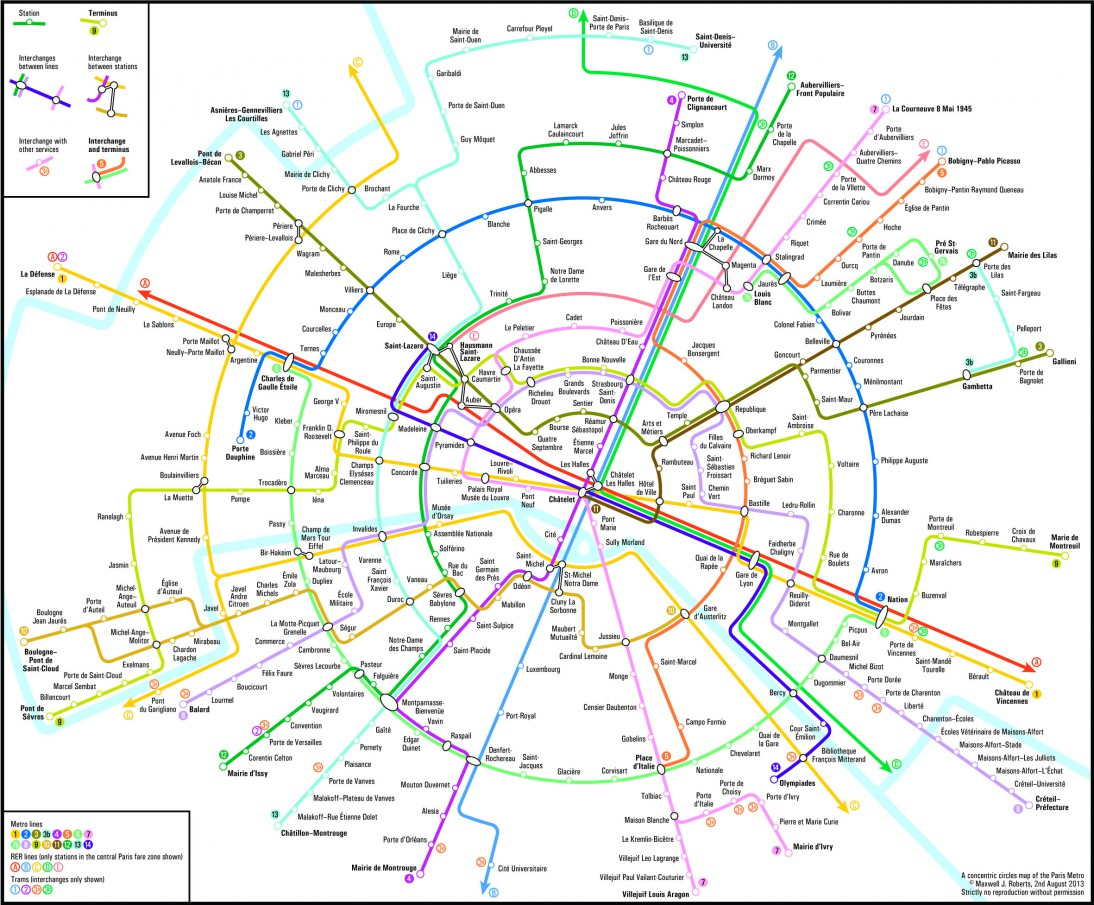
\includegraphics[width=4cm]{fig_0} \\
\textit{Représentation ciculaire du métro parisien}
}%figues de la page de garde


\input{\repRel/Style/pagegarde_cours_minitoc}
\setlength{\columnseprule}{.1pt}

\vspace{2cm}
\pagestyle{fancy}
\thispagestyle{plain}

%Thème : Tris.




\section{Parcours de graphe}
Une fois que nous sommes en présence d'un graphe, il va falloir le parcourir pour répondre à différentes questions : 
\begin{itemize}
\item est-il possible de joindre un sommet $A$ et un sommet $B$ ?
\item est-il possible, depuis un sommet, de rejoindre tous les autres sommets du graphe ?
\item peut-on détecter la présence de cycle ou de circuit dans un graphe ?
\item quel est le plus court chemin pour joindre deux sommets ?
\item \textit{etc.}
\end{itemize}

Les deux algorithmes principaux sont les suivants :
\begin{itemize}
\item le parcours en largeur -- \textit{Breadth-First Search} (BFS) -- pour lequel on va commencer par visiter les sommets les plus proches du sommet initial (sommets de niveau 1), puis les plus proches des sommets de niveau 1 \textit{etc.};
\item le parcours en profondeur  -- \textit{Depth-First Search} (DFS) -- pour lequel on part d'un sommet initial jusqu'au sommet le plus loin. On remonte alors la pile pour explorer les ramifications.
\end{itemize}

Une des difficultés du parcours de graphe est d'éviter de tourner en rond. C'est pour cela qu'on mémorisera l'information d'avoir visité ou non un sommet. 

\subsection{Parcours en largeur}

\subsubsection{Un premier algorithme}
On propose ci-dessous un algorithme de parcours en largeur en utilisant un graphe implémenté sous forme de liste d'adjacence ainsi qu'un sommet \texttt{s} de départ. 

\begin{lstlisting}
def bfs(G:dict, s:str) -> None:
    """
    G : graphe sous forme de dictionnaire d'adjacence
    s : sommet du graphe (Chaine de caractere du type "S1").
    """
    visited = {}
    for sommet,voisins in G.items():
        visited[sommet] = False
    # Le premier sommet à visiter entre dans la file
    file = deque([s])
    while len(file) > 0:
        # On visite la tête de file
        tete = file.pop()
        # On vérifier qu'elle n'a pas été visitée
        if not visited[tete]:
            # Si on l'avait pas visité, maintenant c'est le cas :)
            visited[tete] = True            
            # On met les voisins de tete dans la file
            for v in G[tete]:
                file.appendleft(v)
\end{lstlisting}

Dans cet algorithme : 
\begin{itemize}
\item on commence par créer une liste ayant pour taille le nombre de sommets. Cette liste va permettre de savoir si un sommet a été visité ou non;
\item dans la file, on va commencer par ajouter le sommet initial;
\item on commence alors à traiter la file en extrayant l'indice du sommet initial;
\item si ce sommet n'a pas été visité, il devient visité;
\item on ajoute alors dans la file l'ensemble des voisins du sommet initial;
\item on continue alors de traiter la file. 
\end{itemize}

\begin{rem}
En l'état, à quoi sert cet algorithme ?
\end{rem}


\subsubsection{Applications}
\begin{exemple}
\textit{Comment connaître la distance d'un sommet \texttt{s} aux autres?}
\ifprof
\begin{lstlisting}
def distances(G, s):
    dist = [-1]*len(G)
    q = deque([(s, 0)])
    while len(q) > 0:
        u, d = q.pop()
        if dist[u] == -1:
            dist[u] = d
            for v in G[u]:
                q.appendleft((v, d + 1))
    return dist
\end{lstlisting}
\else
\vspace{5cm}
\fi
\end{exemple}

\begin{exemple}
\textit{Comment connaître un plus court chemin d’un sommet s à un autre ? }
\ifprof
\begin{lstlisting}
def bfs(G, s):
    pred = [-1]*len(G)
    q = deque([(s, s)])
    while len(q) > 0:
        u, p = q.pop()
        if pred[u] == -1:
            pred[u] = p
            for v in G[u]:
                q.appendleft((v, u))
    return pred
    
def path(pred, s, v):
    L = []
    while v != s:
        L.append(v)
        v = pred[v]
    L.append(s)
    return L[::-1] # inverse le chemin
\end{lstlisting}
\else
\vspace{10cm}
\fi
\end{exemple}

%\subsubsection{Marquage de sommet}

\subsection{Parcours en profondeur}
\subsubsection{Un premier algorithme}

On propose ci-dessous un algorithme de parcours en profondeur en utilisant un graphe implémenté sous forme de liste d'adjacence ainsi qu'un sommet \texttt{s} de départ. 

\begin{lstlisting}
def dfs(G, s): #
    visited = [False]*len(G)
    pile = [s]
    while len(pile) > 0:
        u = pile.pop()
        if not visited[u]:
            visited[u] = True
            for v in G[u]:
                pile.append(v)
\end{lstlisting}

Dans cet algorithme : 
\begin{itemize}
\item on commence par créer une liste ayant pour taile le nombre de sommets. Cette liste va permettre de savoir si un sommet a été visité ou non;
\item dans la pile, on va commencer par ajouter le sommet initial;
\item on commence alors à traiter le sommet initial après l'avoir extrait de la pile;
\item si ce sommet n'a pas été visité, il devient visité;
\item on ajoute alors dans la pile l'ensemble des voisins du sommet initial;
\item on continue alors de traiter la pile. 
\end{itemize}
À la différence du parcours en largeur, lorsqu'on va traiter la pile, on va s'éloigner du sommet initial... avant d'y revenir quand toutes les voies auront été explorées. 

\subsubsection{Applications}
\begin{exemple}
\textit{Lister les sommets dans l'ordre de leur visite.}
\end{exemple}


\begin{exemple}
\textit{Comment déterminer si un graphe non orienté est connexe ?}
\end{exemple}


\begin{exemple}
\textit{Comment déterminer si un graphe non orienté contient un cycle ?}
\end{exemple}

\section*{Références}

\begin{itemize}
\item Cours de Quentin Fortier \url{https://fortierq.github.io/itc1/}.
\item Cours de JB Bianquis. Chapitre 5 : Parcours de graphes. Lycée du Parc. Lyon.
\item Cours de T. Kovaltchouk. Graphes : parcours. Lycée polyvalent Franklin Roosevelt, Reims.
\item \url{https ://perso.liris.cnrs.fr/vincent.nivoliers/lifap6/Supports/Cours/graph_traversal.html}
\item \url{http ://mpechaud.fr/scripts/parcours/index.html}
\end{itemize}